% Dr. Nam H. Le. drnamlabs.com, bunnyquant.com
% Cell Systems format: Summary, Highlights, In Brief, Results, Discussion with an
% explicit limitations section, then STAR Methods.
\documentclass[11pt]{article}

\usepackage[margin=1in]{geometry}
\usepackage[utf8]{inputenc}
\usepackage[T1]{fontenc}
\usepackage{times}
\usepackage{graphicx}
\usepackage{booktabs}
\usepackage{amsmath,amssymb}
\usepackage{xcolor}
\usepackage{caption}
\usepackage{enumitem}
\usepackage{microtype}
\usepackage[numbers,sort&compress]{natbib}
\usepackage[colorlinks=true,allcolors=blue!55!black]{hyperref}

\graphicspath{{figures/}}
\captionsetup{font=small,labelfont=bf}
\setlength{\parskip}{0.3em}
\renewcommand{\baselinestretch}{1.12}

\newcommand{\goal}[1]{\textit{``#1''}}

\title{\vspace{-2em}\textbf{Most of it was toxicity: a request-blind baseline reproduces
language-conditioned phenotype prediction in Cell Painting}}

\author{Nam H. Le\,$^{1,2,*}$\\[0.4em]
\small $^{1}$Department of Computer Science, University of Vermont, Burlington, VT, USA\\
\small $^{2}$Lead contact\\
\small $^{*}$Correspondence: \texttt{nam.le@uvm.edu}}

\date{}

\begin{document}
\maketitle
\vspace{-2.5em}

\section*{Summary}

Image-based profiling archives are indexed by the perturbation applied, not by the
cellular state produced, so re-using them to answer a new question usually means a new
screen. We asked whether such an archive can instead be addressed by outcome, stated in
ordinary language, and built a system that maps an English description of a desired
cellular appearance to a compound, a dose, and a refusal when the library contains
nothing suitable. On RxRx3-core it reached an area under the curve (AUC) of
$0.842/0.873$ on compounds whose chemical scaffold it had never seen. Scoring the same
predictions with a baseline that never reads the request, constructed from the model's
own prediction for \goal{kill most of the cells}, gave $0.833/0.855$. The cause is that
per-cell features are averaged over segmented survivors, so dying cells read brighter
per unit area: against a 3.5\% base rate of cell loss, 64--69\% of wells satisfying a
per-cell \goal{brighter} predicate had also lost cells. Redefining each predicate to
require surviving cells lowers the headline to $0.799/0.861$ and multiplies the margin
over that baseline tenfold. The same confound recurs in L1000 transcriptomics as a
nonspecific response. Retrieval by example in a learned image representation outperforms
the model wherever candidates have already been imaged, but scores them using measurements
that define their own labels, so the two answer different questions. We propose that a
request-blind baseline, and a statement of whether a baseline can see the label's own
measurement, be reported alongside every result in this setting.

\section*{Highlights}
\begin{itemize}[leftmargin=1.2em,itemsep=0.15em]
\item A request-blind baseline scores 0.833 where a goal-conditioned model scores 0.842
\item Per-cell features average over survivors: 64--69\% of ``brighter'' wells lost cells
\item Requiring survival lowers accuracy but multiplies the real margin tenfold
\item The confound recurs in L1000 as nonspecific response, at 78--86\%
\item Retrieval by example wins, but detects the label rather than predicting it
\end{itemize}

\section*{In brief}

Le shows that per-cell morphological features in Cell Painting are entangled with cell
death strongly enough that a baseline ignoring the request matches a language-conditioned
model trained to answer it. Redefining predicates to require surviving cells lowers
headline accuracy while revealing the genuine, smaller effect, and the same confound
appears in transcriptomic profiling.

\vspace{0.5em}
\noindent\textbf{Keywords:} image-based profiling; Cell Painting; high-content screening;
phenotypic drug discovery; benchmark design; confounding; selective prediction;
dose response; CellProfiler; LINCS

\section{Introduction}

A phenotypic screen produces a decision and an archive. The decision is used; the archive
usually is not, because it is indexed by what was done to the cells rather than by what
the cells did. If a screen was run to find compounds that kill a cancer line, its images
also record every other morphological consequence of those compounds, and nobody can
retrieve them, because the question ``which of these made the mitochondria dimmer without
killing anything'' was never asked and therefore never labelled.

Image-based profiling has made such archives large and public
\citep{bray2016cellpainting,weisbart2024gallery,chandrasekaran2023jump,kraus2025rxrx3core},
and recent work aligns their images with text that describes the perturbation applied
\citep{lu2025cellclip,ilyosbekov2026morphoclip}. That direction is forward: given a
treatment, find its images, or given images, name the treatment. The inverse direction,
from a desired outcome to the intervention that produces it, is the one a screening group
would use, and it changes the problem in two ways. There is no text to align with, because
the desired outcome was never recorded, so the supervision must be manufactured from
measurements made for other purposes. And the correct answer includes a dose, because the
concentration that produces an effect strongly is often the concentration that kills.

Manufacturing supervision makes the \emph{definition} of success a modelling decision
rather than a formality, and this paper is mostly about the consequences of getting that
definition wrong. We built a system that reads an English request and returns ranked
(compound, dose) pairs with a dose-response curve, or declines. It performed well. It then
turned out that almost all of its apparent skill was a single confound, invisible in the
headline metric and detectable with a control that costs nothing.

The coupling itself is not new: image-based morphology predicts cell-health readouts
accurately \citep{way2021cellhealth}, and that is a useful result in its own right. What we
report is that the coupling silently redefines what a goal-conditioned benchmark measures,
while \emph{improving} its headline number, so that a model is rewarded for learning the
confound. That a model can score well for a reason unrelated to the stated task is a
recurring hazard in scientific machine learning
\citep{chuang2018adversarial,wallach2018memorization,geirhos2020shortcut}; our contribution
is a specific, free control for this data type and a redefinition that removes the
confound at a measurable cost in apparent accuracy.

\section{Results}

\subsection{A phenotype archive addressed by outcome}

RxRx3-core \citep{kraus2025rxrx3core} contains 56,700 query-compound wells covering 1,671
compounds at eight concentrations from 0.0025 to 10\,$\mu$M, imaged in six fluorescent
channels in human umbilical vein endothelial cells across four experiments and 160 plates.
The unit of analysis throughout is the \emph{group}: one (compound, dose) pair summarised
as the median over its replicate wells, giving 13,350 groups.

We defined eight measurements, each the simplest available statement of one behaviour that
can be phrased in plain language: cell eccentricity, nucleus area, mean Hoechst in the
nucleus, mean MitoTracker and mean phalloidin in the cell, the outer-quartile radial
fraction of phalloidin, and the median absolute deviation and mean of the wheat-germ
agglutinin channel. Every well was scored as a robust $z$ against the query wells of its
own plate (STAR Methods). Cell loss has no single CellProfiler column, so it was measured
from the images as total nuclear foreground divided by the median area of a single nucleus,
normalised to the plate (Figure~\ref{fig:data}).

A predicate is a probability rather than a class,
$p = \sigma\!\left((s\,z - \tau)/T\right)$ with $\tau = 2.0$ and $T = 0.5$ fixed before any
model was trained and never tuned; missing measurements propagate as NaN and are masked. A
request is an English sentence paired with a conjunction of predicates; the sentence is all
the model reads, and the formula is used only to build the label and score the answer. The
set contains 259 requests under the definition developed below, split into training,
unseen phrasings of trained concepts (26), unseen concepts formed by conjunction or
negation (38), and requests that no (compound, dose) group in the archive satisfies (37),
the last determined by measurement rather than by judgement.

\begin{figure}[t]
\centering
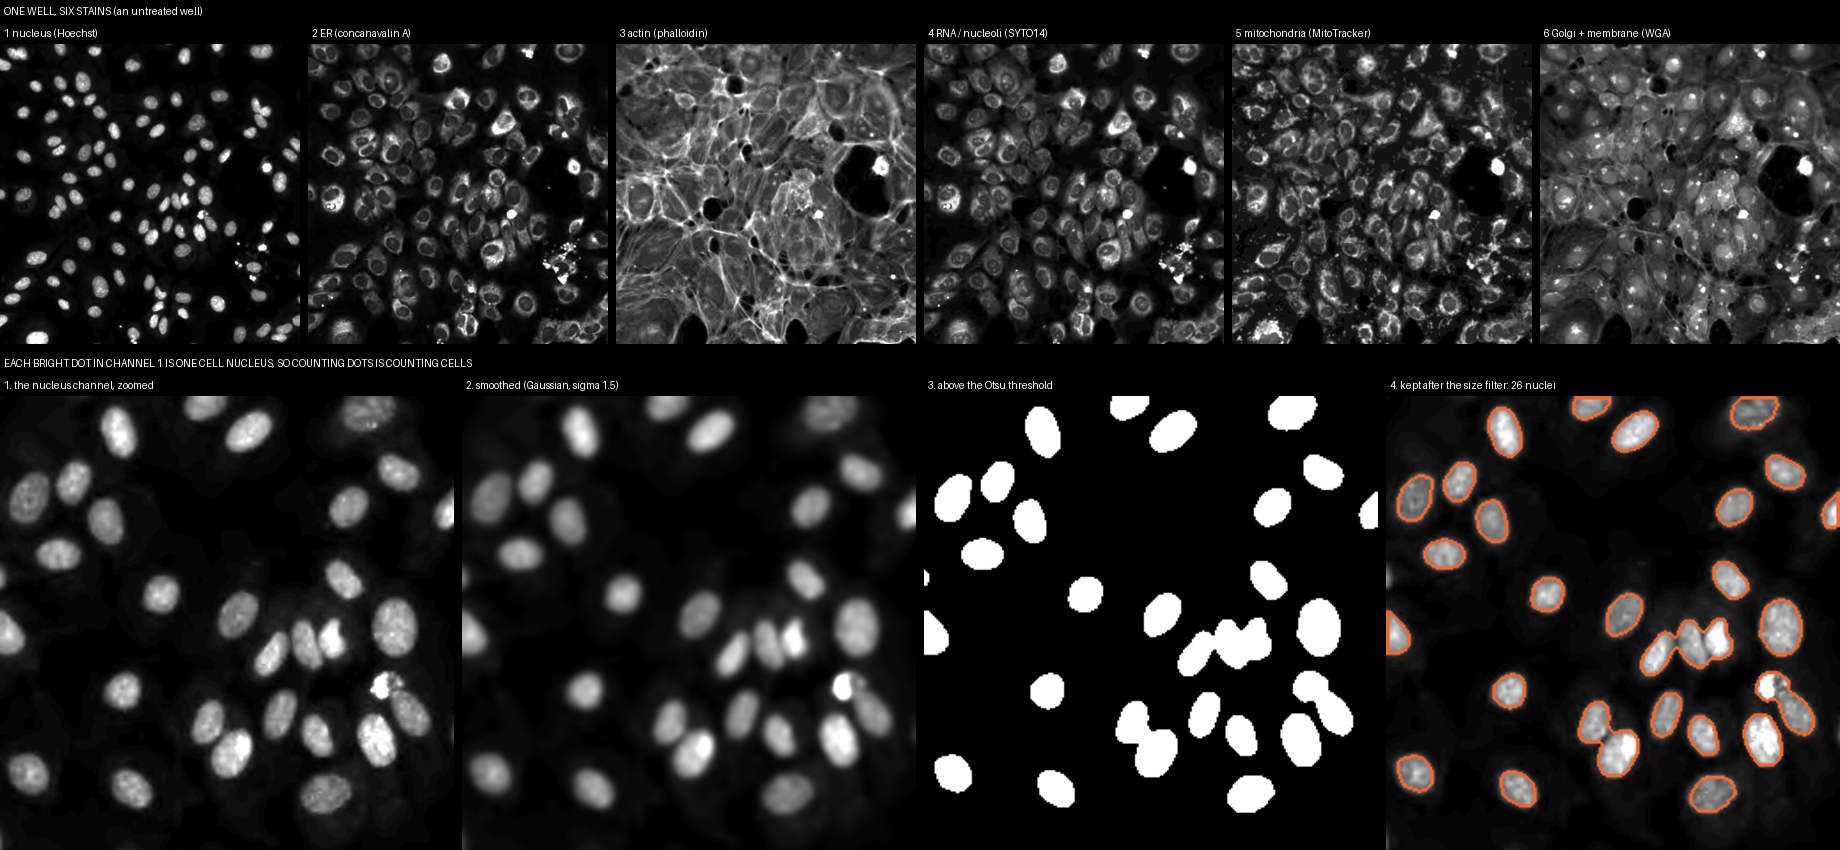
\includegraphics[width=\textwidth]{01_what_is_a_dot.png}
\caption{\textbf{From images to measurements.} Top: one well in six channels. Bottom: the
nucleus channel, smoothed, thresholded, and filtered by size. Objects are counted as total
nuclear area divided by the median area of one nucleus rather than as connected components,
because at high density nuclei merge and component counting undercounts in precisely the
wells where cell loss matters. Both panels of any treated-versus-reference comparison are
mapped by a single brightness scale taken from the reference; contrast-stretching each
image against its own percentiles destroys the comparison.}
\label{fig:data}
\end{figure}

\subsection{A baseline that never reads the request}

Given a trained goal-conditioned model, take its prediction for one fixed request,
\goal{kill most of the cells}, and use that single vector of scores to rank candidates for
every other request. The resulting scorer is blind to the question. A second, equally cheap
control ranks by concentration alone. Both are free once a model exists.

Compounds were split by Bemis-Murcko scaffold \citep{bemis1996scaffold} into 70/10/20, so a
test compound shares no ring skeleton with any training compound; splitting at random
places salts and close analogues on both sides and reports interpolation
\citep{wallach2018memorization}. Numbers are five-seed ensembles.

Under the literal reading of the per-cell features, the system reached AUC $0.842$ on
unseen phrasings and $0.873$ on unseen concepts. The request-blind baseline reached
$0.833$ and $0.855$. The behaviour-specific contribution was $+0.010/+0.018$
(Table~\ref{tab:main}, Figure~\ref{fig:baselines}). Read without the control, this is a
respectable phenotype model; read with it, it is a cytotoxicity detector with a language
interface.

\begin{table}[t]
\centering
\small
\begin{tabular}{lcccc}
\toprule
 & \multicolumn{2}{c}{\textbf{Survival-conditioned}} & \multicolumn{2}{c}{Literal} \\
\cmidrule(lr){2-3}\cmidrule(lr){4-5}
AUC, unseen scaffolds & unseen phrasing & unseen concept & unseen phrasing & unseen concept \\
\midrule
goal-conditioned model   & \textbf{0.799} & \textbf{0.861} & 0.842 & 0.873 \\
request-blind baseline   & 0.696 & 0.789 & 0.833 & 0.855 \\
dose-only baseline       & 0.722 & 0.761 & 0.758 & 0.775 \\
\midrule
margin over request-blind & \textbf{+0.104} & \textbf{+0.072} & +0.010 & +0.018 \\
\bottomrule
\end{tabular}
\caption{\textbf{The same system under both predicate definitions.} The literal definition
produces a higher headline and almost no margin over a scorer that ignores the request.
Requiring the cells to survive lowers the headline and multiplies the margin by ten. On
compounds it has seen, the model reaches $0.929/0.969$, so the bottleneck is chemistry to
phenotype rather than language or capacity.}
\label{tab:main}
\end{table}

\subsection{Per-cell features are entangled with cell death}

CellProfiler \citep{carpenter2006cellprofiler} reports per-cell features as averages over
the objects it can segment, which are the cells still present. A dying cell rounds up and
condenses and therefore reads brighter per unit area. The entanglement is directly
measurable. Against a base rate of 3.5\% of groups showing cell loss, the share of groups
satisfying a per-cell predicate that had also lost cells was 69\% for brighter DNA, 66\%
for brighter actin, 64\% for brighter mitochondria, 62\% for smaller nuclei, 56\% for
fainter actin, 49\% for bigger nuclei, 42\% for dimmer mitochondria, 37\% for dimmer DNA,
and 16\% for elongation (Figures~\ref{fig:wells} and \ref{fig:confound}).

So \goal{make the mitochondria brighter}, read literally off the features, is substantially
a synonym for \goal{kill the cells}. A model fitted to that target learns the shortcut
because the shortcut is what the label says.

\begin{figure}[t]
\centering
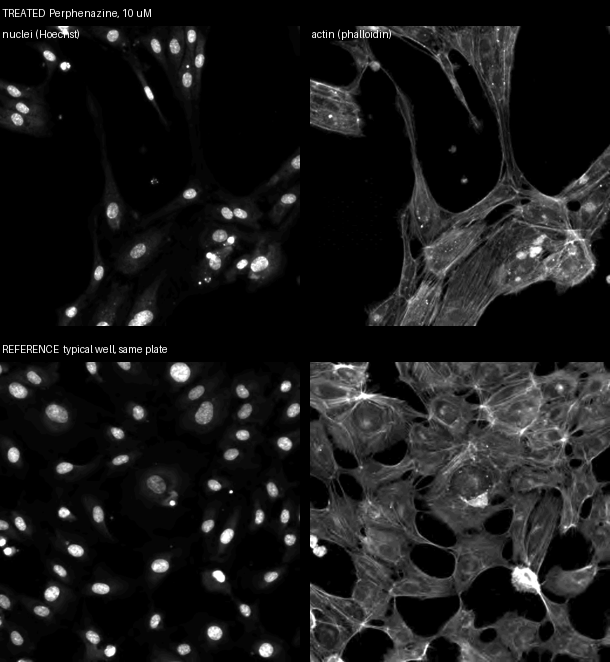
\includegraphics[width=0.62\textwidth]{01_wells.png}
\caption{\textbf{The confound before it is a number.} One treated well above a typical well
from the same plate, two of the six channels, native resolution, one brightness scale per
channel taken from the reference. Most cells are gone and those remaining are rounded and
bright; a per-cell average is taken over the survivors in the top row.}
\label{fig:wells}
\end{figure}

\begin{figure}[t]
\centering
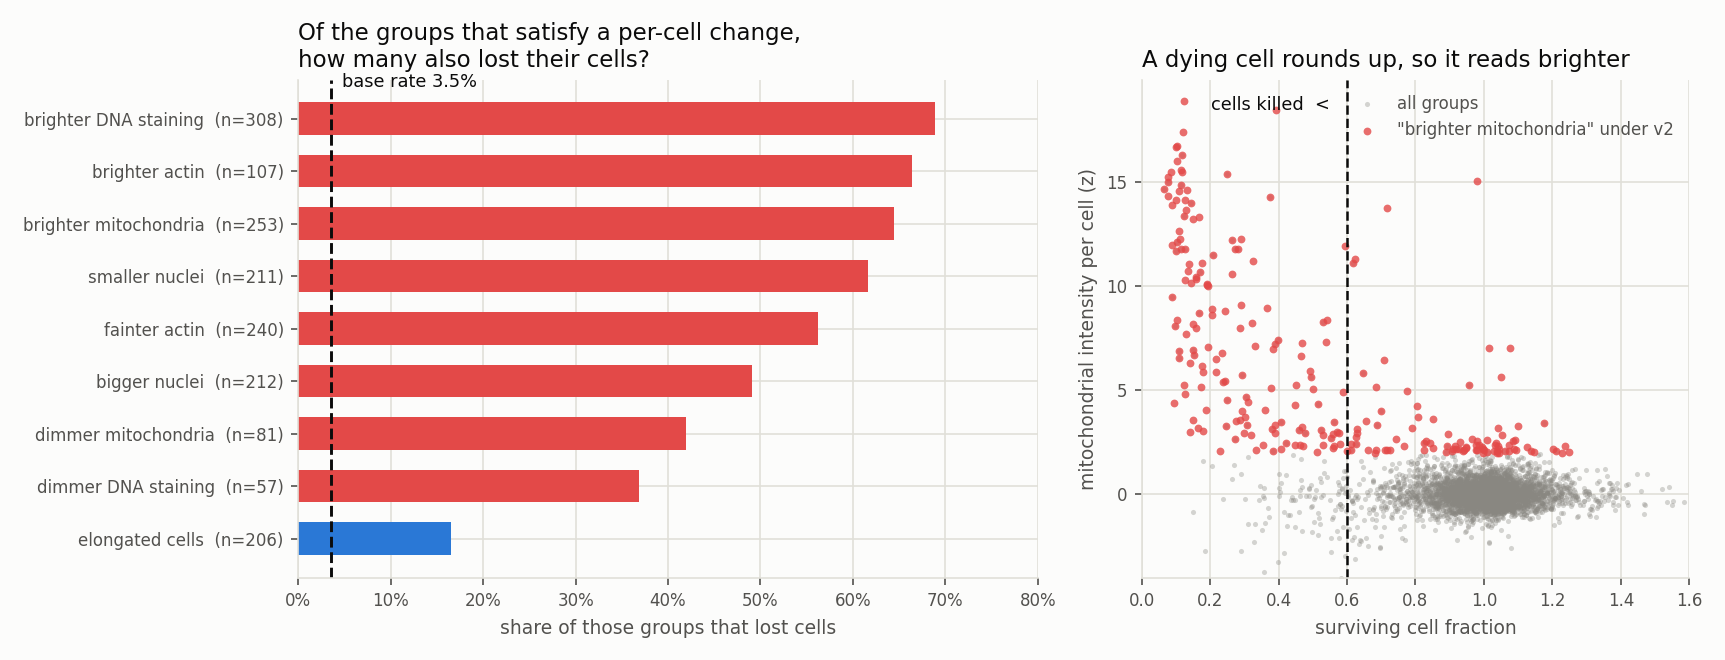
\includegraphics[width=\textwidth]{03_the_definition_problem.png}
\caption{\textbf{Quantifying the entanglement.} (Left) For each per-cell predicate, the
share of satisfying groups that also lost cells, against the 3.5\% base rate (dashed).
Only elongation is close to clean. (Right) Per-cell mitochondrial intensity against
surviving fraction; groups satisfying the literal predicate concentrate where the cells
have gone.}
\label{fig:confound}
\end{figure}

We therefore define every per-cell predicate as a conjunction, \emph{$X$ holds in the
measured cells and the cells were not killed}, with one exception: a request that itself
asks for cell loss keeps the literal meaning, since there is nothing left to protect.
Under this definition the set of requests that nothing in the archive satisfies grows from
25 to 37, because conjunctions such as \goal{bigger nuclei and brighter mitochondria} occur
only in dying cells. The headline falls and the margin over the request-blind baseline
rises tenfold (Table~\ref{tab:main}).

\subsection{The response exists in a dose window}

The output is deliberately non-monotone in dose,
\begin{equation}
p \;=\; \underbrace{\sigma(b_0 + b_1 z)}_{\text{effect rises}}\cdot
        \underbrace{\sigma(c_0 - \operatorname{softplus}(b_3)\,z)}_{\text{survival falls}},
\label{eq:window}
\end{equation}
where $z$ is the standardised $\log_{10}$ dose. This is not decoration. Under the
survival-conditioned definition, 60 of the 80 compounds that brighten mitochondria in
living cells anywhere in the archive peak \emph{below} the top dose, because the top dose
kills (Figure~\ref{fig:window}). A monotone output cannot represent a dose window and
prefers the toxic compound.

\begin{figure}[t]
\centering
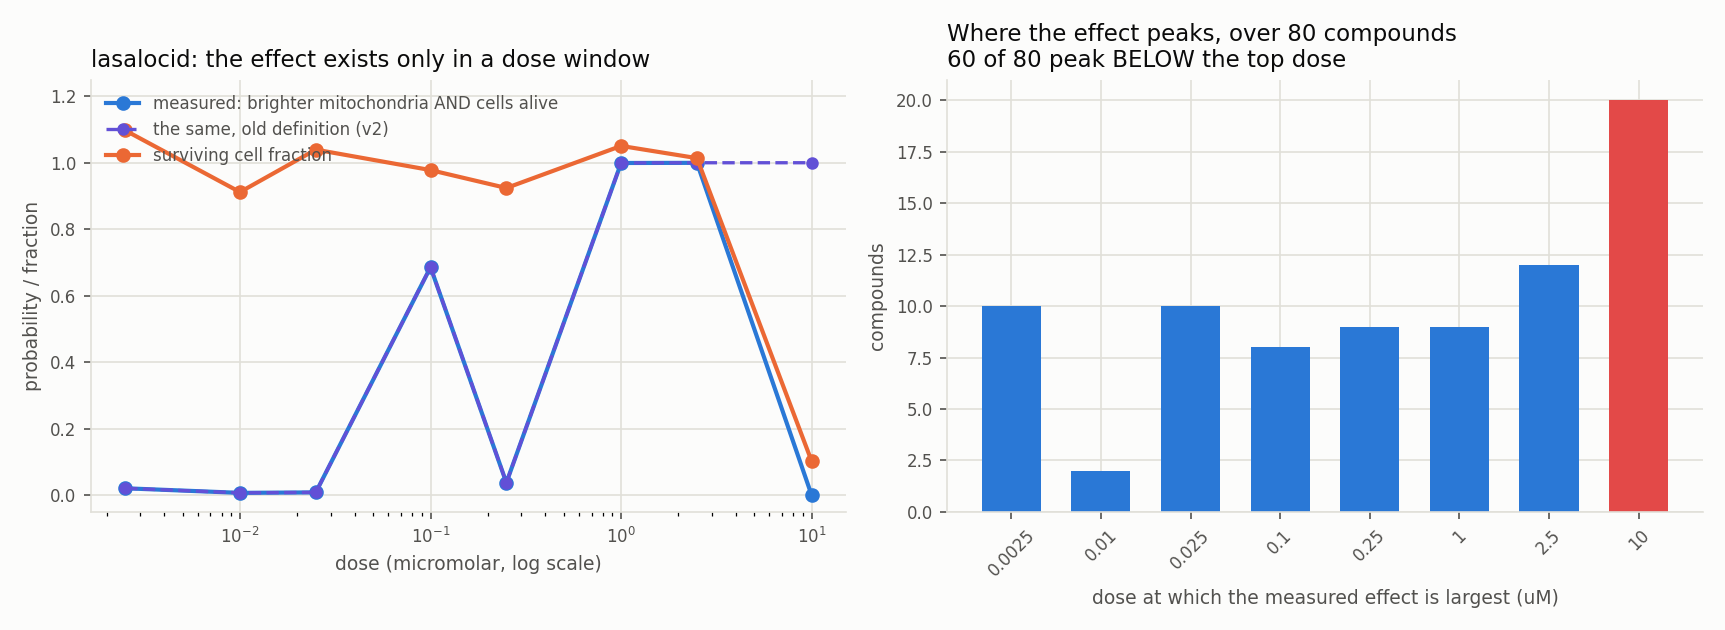
\includegraphics[width=\textwidth]{04_dose_window.png}
\caption{\textbf{Why the output is non-monotone.} (Left) One compound's measured
probability of brighter mitochondria in living cells, its literal counterpart, and its
surviving fraction, against dose. (Right) For the 80 compounds that satisfy the
survival-conditioned predicate anywhere, the dose at which the measured effect is largest;
60 peak below the top dose.}
\label{fig:window}
\end{figure}

\subsection{Declining is a scored output}

A system that always answers cannot be used for screening. Over 37 requests that nothing in
the archive satisfies against 64 that something does, the model's own confidence separates
them at AUC $0.85$. At a threshold calibrated on validation compounds it answers 89\% of
answerable requests and wrongly answers 38\% of impossible ones.

Two details of that measurement are themselves transferable. The confidence statistic is
the mean of the top ten scores, not the maximum: a maximum is an extreme-value statistic
that grows with the size of the candidate pool, so a threshold learned on one pool does not
transfer to a larger one and a single lucky candidate suffices to answer an impossible
request. Going from 1,256 to 2,670 candidate groups, the median maximum for impossible
requests rose from $0.038$ to $0.083$ while the achievable ones did not move; refusal AUC
is $0.85$ with the top-ten mean and $0.792$ with the maximum. And calibrating the threshold
on \emph{training} compounds, where the model fits closely, produced a threshold that
answered only 16\% of answerable requests.

\begin{figure}[t]
\centering
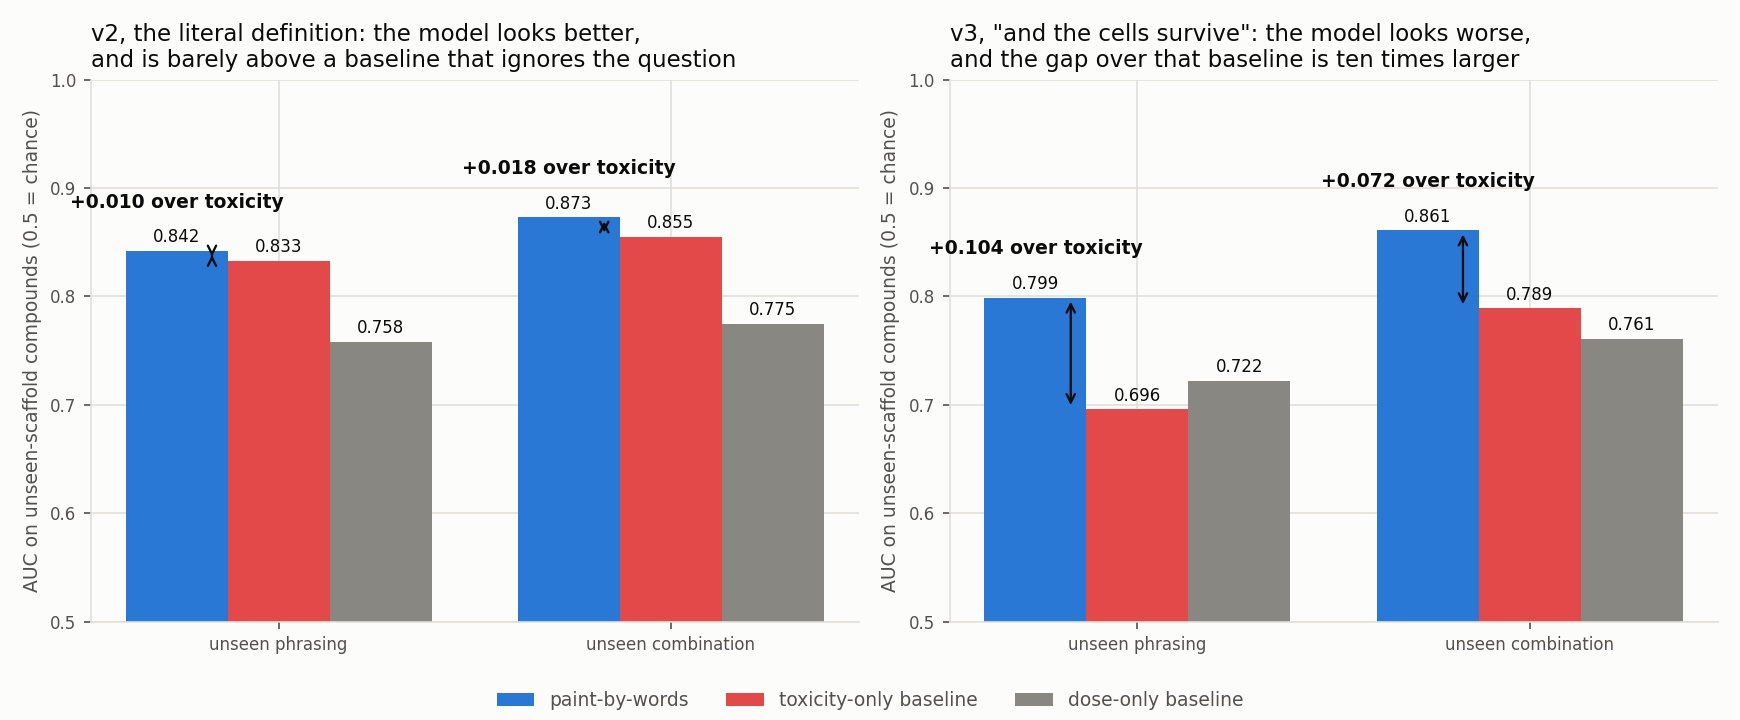
\includegraphics[width=\textwidth]{05_against_the_baselines.png}
\caption{\textbf{Both definitions, against both baselines.} Bars begin at 0.5, which is
chance. Under the literal definition the model sits almost on top of a scorer that ignores
the request. Under the survival-conditioned definition it scores lower and the gap is ten
times larger.}
\label{fig:baselines}
\end{figure}

\subsection{What the ranking saves, counted in wells}

AUC states how a ranking is ordered, not what a screen costs. For 64 held-out requests on
unseen scaffolds, 38 of them conjunctions whose concept was never trained, we asked how
often a budget of $k$ wells contains a real hit (Figure~\ref{fig:budget}).

Random order needs a median of 267 wells to reach a first hit and the model needs 12. The
request-blind baseline needs 18, so most of that reduction is general activity rather than
goal-specific skill, and at a budget of 48 wells ranking by dose alone outperforms the
model (73\% against 67\%). Goal-specific skill survives in two places. At eight wells, one
row of a 96-well plate, the model satisfies 42\% of requests against 20\%: paired over the
same requests, $+22\%$, 95\% CI $[+11\%, +33\%]$, with 15 requests satisfied only by the
model against 1 only by the baseline, McNemar $p = 0.0005$. At 384 wells it reaches 98\%
against 81\%, so roughly one request in five is unreachable along the toxicity route at any
budget. Between 16 and 96 wells the two are not separable (at 16 wells, $+11\%$,
$p = 0.12$), and we report that null because it bounds the claim.

\begin{figure}[t]
\centering
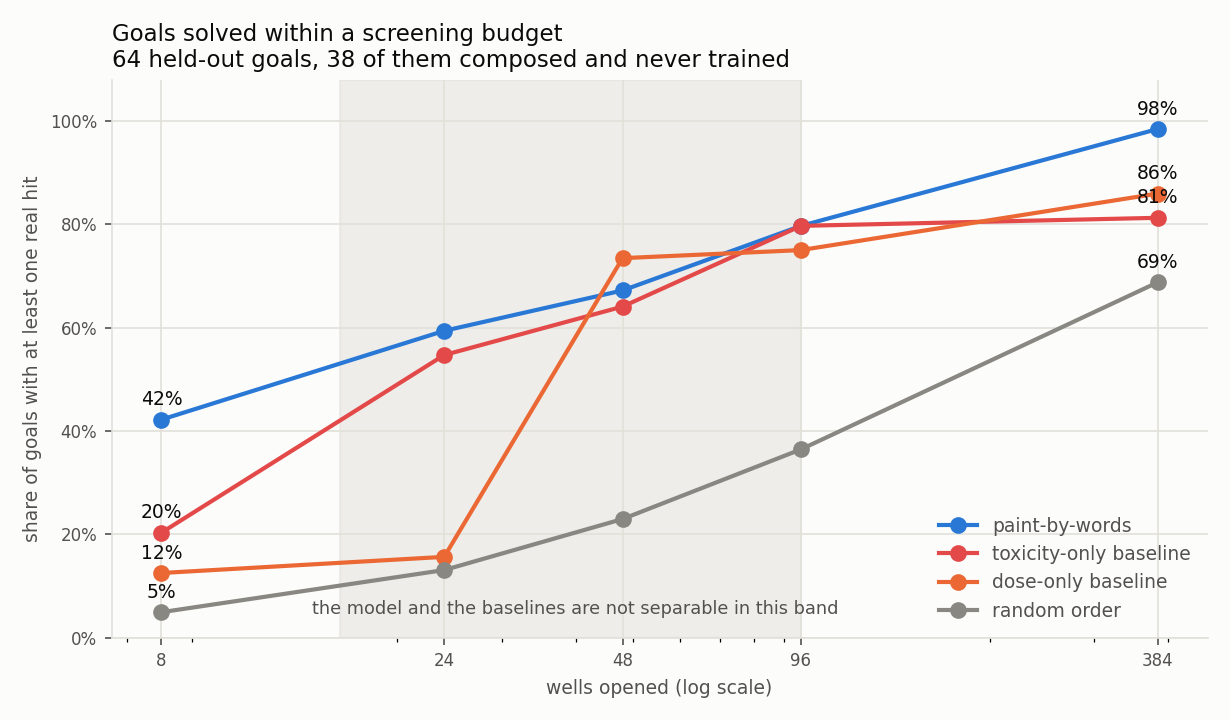
\includegraphics[width=0.92\textwidth]{06_screening_budget.png}
\caption{\textbf{Requests satisfied within a screening budget.} The advantage over trivial
baselines is confined to very small budgets and to the ceiling; in the shaded band the
curves are not separable, and at one budget the dose-only baseline wins outright.}
\label{fig:budget}
\end{figure}

\subsection{Retrieval by example answers a different question, and a leakage control shows it}

Before claiming that stating a goal in language is useful, it must be compared with the
obvious alternative that uses no language at all: point at wells that already do what you
want, average their learned image representation, and rank every other well by similarity.
We ran exactly that, using the OpenPhenom representation that the archive's publisher
distributes, with prototypes built only from training-scaffold groups and scored on the
same unseen-scaffold groups and the same held-out requests as the model.

Retrieval wins, and not narrowly: AUC $0.918$ on unseen concepts and $0.851$ on unseen
phrasings, against $0.861$ and $0.799$ for the goal-conditioned model, which beats it on
only 13 of 64 requests (median difference $-0.044$). Five example wells suffice; the
five-shot prototype matches the one built from every training positive
(Table~\ref{tab:retrieval}).

That comparison, however, is not between two solutions to one problem. Retrieval scores a
candidate group using measurements taken \emph{on that same group}, and the label of that
group is a function of those measurements. Running the identical retrieval on the eight
engineered features from which the labels are themselves computed makes the point
quantitative: it reaches $0.966/0.961$. We report that arm as a \emph{leakage control}
rather than as a competitor, because at that point the score is the label being read back
rather than inferred, and it bounds how much of any image-space retrieval score is the
same thing.

The distinction is therefore detection versus prediction. Retrieval requires the candidate
to have been imaged, and its ceiling is the reliability of the measurement; the
goal-conditioned model maps a sentence, a structure and a dose to a probability, and can
score a compound that has never been run. Where an archive is being re-mined and every
candidate is already imaged, retrieval by example is the right tool and our contribution is
the predicate definition and the evaluation protocol rather than the ranker. Where the
question is which compound to image next, retrieval has no entry.

\begin{table}[t]
\centering
\small
\begin{tabular}{lcc}
\toprule
AUC on unseen-scaffold groups & unseen phrasing & unseen concept \\
\midrule
retrieval by example, OpenPhenom, all training positives & \textbf{0.851} & \textbf{0.918} \\
retrieval by example, OpenPhenom, five examples & 0.848 & 0.918 \\
goal-conditioned model (structure only, never imaged) & 0.799 & 0.861 \\
request-blind baseline & 0.696 & 0.789 \\
\midrule
\textit{leakage control: retrieval on the label's own features} & \textit{0.961} & \textit{0.966} \\
\bottomrule
\end{tabular}
\caption{\textbf{Detection and prediction are not the same axis.} Retrieval by example
outperforms the model, but it scores each candidate using measurements made on that
candidate, and the label is a function of those measurements. The final row runs the same
retrieval on the eight features from which the labels are computed; it is a control for how
much of a retrieval score is the answer being read back, not a method.}
\label{tab:retrieval}
\end{table}

\subsection{A vision-language model as a second measuring instrument}

Replacing the engineered measurement with a vision-language model is an increasingly common
design, so we tested the substitution on the same wells. Two thousand groups were rendered
as a treated panel beside a reference panel from the same plate, six channels, two
native-resolution crops, one brightness scale per channel from the reference, with blind
identifiers. The model returned seven scores from 0 to 100 with 50 meaning no difference.
Calibration was label-free, so the physical measurements were never used to fit it, and the
calibrated scores then drove the same predicate formulas. Only the instrument differed.

Agreement with the measurements, behaviour by behaviour, was 0.93 for cell loss, 0.87 for
elongation, 0.81 for dimmer DNA, 0.75 for dimmer mitochondria, 0.74 for fainter actin,
0.73 for brighter actin, 0.69 for brighter mitochondria, 0.66 for bigger nuclei, 0.59 for
brighter DNA and 0.58 for smaller nuclei. The pattern is interpretable: the judge is
reliable at counting and at gross shape, mediocre at ``dimmer'', and weakest at ``brighter''
and at small size changes.

The decision-level result is worse than the instrument-level one. Trained as a label
source, this branch ranks unseen compounds \emph{below its own} request-blind score
($-0.02/-0.08$ AUC). Doubling the labels from 1,000 to 2,000 groups gained $+0.04$ and
saturated; those 2,000 groups already cover 100\% of the positives that exist in the
archive for these behaviours among training compounds, so the ceiling is the archive rather
than the annotation budget. Test-retest agreement was 0.80--0.93, so the judge was reliable
and invalid at the same time, and a reliability check alone would have endorsed it.

\subsection{The confound recurs in transcriptomic profiling}

To ask whether this is particular to microscopy, we repeated the label analysis on L1000
\citep{subramanian2017lincs}, where the candidate dominant axis is a nonspecific
transcriptional response rather than cell death, quantified by the transcriptional activity
score that the resource already publishes. Using the same predicate constants, the same
robust normalisation, and 14 hallmark gene sets in MCF7 (24,097 signatures), a strong
nonspecific response occurred in 17.4\% of groups but accompanied 86\% of groups with MYC
targets down, 83\% with the hypoxia response up, proliferation down, mTORC1 up or TNF-$\alpha$
up, 82\% with G2/M down, 81\% with apoptosis up, and 78\% with p53 up. The only clean
predicates were the three growth axes, and they are rare (proliferation up, $n = 53$, 15\%;
MYC up, $n = 45$, 9\%; G2/M up, $n = 85$, 8\%).

The shape is the same in both archives. The dominant axis of variation in a compound
library is how much damage the compound did, seen through a microscope in one case and
through a transcriptome in the other.

\section{Discussion}

A benchmark assembled after the fact from measurements made for another purpose inherits
that purpose. Here the inheritance was quantitative: the literal reading of per-cell
morphological features turned a phenotype benchmark into a cytotoxicity detector while
improving its headline number, which is the combination that makes such an error durable.
Nothing about the model was wrong. The label said what the model learned.

Three practices follow, each free once a model has been trained. First, report a
request-blind baseline beside every number: take the model's own prediction for one fixed,
dominant request and score every other request with it. If the margin is small, the
benchmark is measuring the dominant axis rather than the stated task. The dominant axis is
domain-specific, cytotoxicity here and nonspecific stress in transcriptomics, and plausibly
solubility, assay interference or sequence length elsewhere, but the control is the same.
Second, when a language model is used as a judge, validate it per behaviour against an
independent instrument and publish the table rather than a mean; reliability is not
validity. Third, check that any confidence statistic is invariant to the size of the
evaluation pool, because extreme-value statistics are not. Fourth, and most easily missed,
state whether a baseline has access to the measurement that defines the label. A retrieval
baseline scored on wells that have already been imaged is detecting, not predicting, and
running the same retrieval in the feature space the labels are computed from gives the
leakage ceiling, which here was $0.96$. Comparing a detector and a predictor on a single
axis of AUC answers no question that anyone asked.

The positive result that survives these controls is real but modest: about $+0.10$ AUC over
a scorer that ignores the request, a doubled hit rate at an eight-well budget, and access to
roughly one request in five that general cytotoxicity cannot reach. We regard the modesty
as the point. A smaller number that means what it says is more useful than a larger one
that does not, and the difference between them was not visible in the metric.

\subsection*{Limitations of the study}

The system selects from an existing library at doses already run; it does not design
molecules. Every result is retrospective and no prediction has been tested at the bench.
``Unseen'' means unseen chemistry under the same measurement conditions: compounds are held
out by scaffold, but training and test share plates and staining batches, and because 1,661
of 1,671 compounds appear in only one of the four experiments, holding out an experiment
would also hold out its chemistry, so batch transfer is unmeasured here and would require an
archive in which the same compounds are run across sources
\citep{chandrasekaran2023jump}. The behaviours are eight image features and are not claims
about mechanism. All wells are one cell type. Some held-out requests have 3--10 satisfying
groups in the entire archive, where an AUC is a coin flip with a number attached, which is
why the released system reports its support count with every answer. The frozen sentence
encoder does not represent direction, placing \goal{push the actin out to the edge} and
\goal{pull the actin away from the edge} at cosine 0.76, so for such requests the model
answers the opposite question confidently; the released system detects and reports the
condition but does not fix it. Finally, where every candidate has already been imaged,
retrieval by example in a learned representation outperforms the model
(Table~\ref{tab:retrieval}); the goal-conditioned model earns its place only in the regime
where the candidate has not been imaged and retrieval therefore cannot score it.

\subsection*{A pre-registered test}

The single result that would move this work from a retrospective analysis to a validated
instrument is small, and we state it in advance. For each request, two shortlists of eight
wells are sealed before any plate is run, one from the model and one from the request-blind
baseline; wells are run blind and scored by the pre-specified predicate; the hypothesis is
that the model's shortlist contains a real hit for more requests. At the discordance rate
measured here, 80\% power requires approximately 30 requests, that is 480 wells, under two
384-well plates, decided by McNemar's exact test at $\alpha = 0.05$. The assumption carrying
risk is that the discordance rate holds prospectively; a prospective run also introduces a
new batch and so tests batch transfer at the same time.

\section*{STAR Methods}

\subsection*{Key resources}

RxRx3-core \citep{kraus2025rxrx3core}, obtained from the publisher and used under its
end-user licence; it is not redistributed. LINCS L1000 level-5 signatures
\citep{subramanian2017lincs}. MSigDB hallmark gene sets. Software: Python, PyTorch, RDKit
\citep{rdkit}, scikit-learn, SciPy, CellProfiler-derived features as released with the
archive, and the sentence encoder \texttt{nli-mpnet-base-v2}
\citep{reimers2019sbert,song2020mpnet}.

\subsection*{Method details}

\paragraph{Normalisation.} Each well is scored as
$z = (x - \operatorname{median}\mathcal{Q})/(1.4826\,\operatorname{MAD}\mathcal{Q})$, where
$\mathcal{Q}$ is the set of query-compound wells on the same plate. The reference is the
query wells rather than the empty control wells because the archive has no solvent control
and empty wells as reference produced 12--20\% apparent effects in inert wells in a pilot.
The median absolute deviation is used rather than the standard deviation because the
quantity of interest is the tail and a standard deviation is inflated by the outliers being
detected.

\paragraph{Cell counting.} Nuclei are segmented on the Hoechst channel by Gaussian smoothing
($\sigma = 1.5$), Otsu thresholding \citep{otsu1979threshold}, connected-component labelling
and a size filter. The count is total nuclear foreground divided by the median area of one
nucleus, divided in turn by the median count of the query wells on the same plate. Validated
by split-half reproducibility over replicate wells and by a 0.5\% false-positive rate at the
two lowest doses; the 0.6 cut was fixed from that measurement.

\paragraph{Rendering.} For any treated-versus-reference comparison, the brightness scale is
computed once from the reference well and applied unchanged to both, at native resolution.
In an earlier round each panel was contrast-stretched against its own percentiles and the
same vision-language judge scored at chance on four of eight behaviours; a single shared
scale moved those four to AUC 0.81--1.0.

\paragraph{Model and fitting.} A frozen sentence embedding and a chemical representation
(Morgan count fingerprint \citep{rogers2010ecfp} with MACCS keys and standardised RDKit 2D
descriptors) enter a shared trunk that emits the parameters of Equation~\ref{eq:window}.
Each behaviour is sampled as its own task with equal weight. Training uses cross-entropy
against the soft targets and AdamW, with early stopping on held-out \emph{compounds}; no
test compound is seen by the model or by the model-selection rule. Interference between
behaviours was measured rather than assumed (mean gradient cosine on the shared trunk
$\approx 0$, 41--56\% of pairs negative); PCGrad \citep{yu2020pcgrad}, a mixture of experts,
explicit logic heads, a Hill-shaped output and an auxiliary embedding loss each changed
held-out AUC by at most 0.01 and are not used.

\paragraph{Vision-language judge.} Calibration is label-free:
$z = (\text{score} - 50)/(1.4826\,\operatorname{MAD})$ followed by the same fixed-threshold
rule as the measurement branch. Three behaviours received no judge label because a pilot
found the judge at chance on one and reading another through brightness rather than texture.
The exact prompt is released verbatim, since its wording measurably changes the scores.

\subsection*{Quantification and statistical analysis}

AUC is reported per request and averaged over requests, because positives are 1--5\% of
groups and accuracy would be dominated by the base rate. Comparisons between the model and
the request-blind baseline are paired over requests; the eight-well comparison uses
McNemar's exact test, and confidence intervals come from a bootstrap over requests with
5,000 resamples. Reported figures are five-seed ensembles with the scaffold split held
fixed across seeds.

\section*{Resource availability}

\paragraph{Lead contact.} Further information and requests should be directed to the lead
contact, Nam H. Le (\texttt{nam.le@uvm.edu}).

\paragraph{Materials availability.} This study did not generate new materials.

\paragraph{Data and code availability.} The archive is not redistributed. All code, the full
request set with its splits, the evaluation protocol with both trivial baselines printed
beside every number, and the exact prompt given to the vision-language branch are publicly
available at \url{https://github.com/drnamlabs-gif/paint-by-words}. Every figure and number
in this paper is regenerated by a single command in that repository.

\section*{Acknowledgements}

This work was carried out independently and received no specific funding, while the author
held a postdoctoral position at the University of Vermont. We thank the authors of
RxRx3-core for releasing it.

\section*{Declaration of interests}

The author declares no competing interests.

\bibliographystyle{plainnat}
\bibliography{refs}

\end{document}
